Im ersten Teil soll die Schaltung aus \ref{fig:schalt} ohne den Noise-Verstärker
aufgebaut werden. Für $U_{sig}$ wird eine Frequenz von 420$\si{\hertz}$ und eine
Spannung von $27\si{\milli\volt}$ eingestellt. Die Ausgangssignale werden zu
verschiedenen Phasen skizziert.
\begin{figure}[!h]
  \begin{minipage}[t]{0.3\textwidth}
    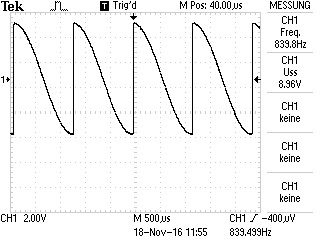
\includegraphics[width=\textwidth]{Bilder/15.jpeg}
    \label{fig:15}
    \caption{\Phi=15\si{\degree}}
  \end{minipage}
  \hspace{12pt}
  \vspace{5pt}
  \begin{minipage}[t]{0.3\textwidth}
    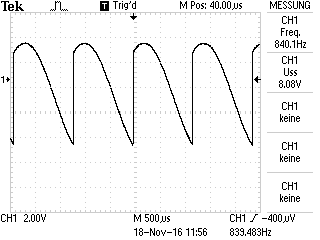
\includegraphics[width=\textwidth]{Bilder/45.jpeg}
    \label{fig:45}
    \caption{\Phi=45\si{\degree}}
  \end{minipage}
  \hspace{12pt}
  \vspace{5pt}
  \begin{minipage}[t]{0.3\textwidth}
    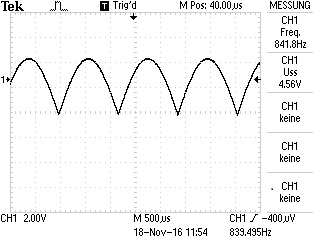
\includegraphics[width=\textwidth]{Bilder/105.jpeg}
    \label{fig:105}
    \caption{\Phi=15\si{\degree}}
  \end{minipage}
  \hspace{12pt}
  \vspace{5pt}
  \begin{minipage}[t]{0.3\textwidth}
    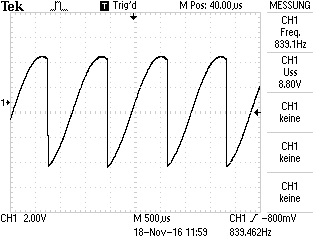
\includegraphics[width=\textwidth]{Bilder/165.jpeg}
    \label{fig:165}
    \caption{\Phi=45\si{\degree}}
  \end{minipage}
  \hspace{12pt}
  \vspace{5pt}
  \begin{minipage}[t]{0.3\textwidth}
    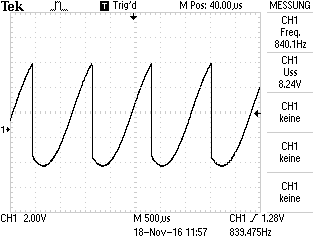
\includegraphics[width=\textwidth]{Bilder/225.jpeg}
    \label{fig:105}
    \caption{\Phi=15\si{\degree}}
  \end{minipage}
  \hspace{12pt}
  \vspace{5pt}
  \begin{minipage}[t]{0.3\textwidth}
    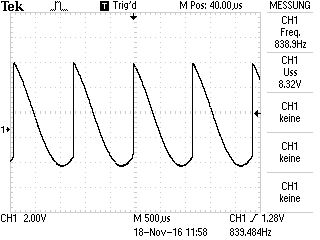
\includegraphics[width=\textwidth]{Bilder/330.jpeg}
    \label{fig:330}
    \caption{\Phi=45\si{\degree}}
  \end{minipage}
  \hspace{12pt}
  \vspace{5pt}
\end{figure}
